\documentclass{beamer}
\newcommand{\myfont}{\rmfamily\normalsize\upshape\mdseries}
\newcommand{\degree}{^\circ}
\newcommand{\R}{\mathbb{R}}

\title{\sffamily Review VI(Slides 333 - 365)}
\subtitle{\textbf{Vector Space \& Sequence of Functions}\\ }
\institute[UM-SJTU JI]{University of Michigan-Shanghai Jiao Tong University Joint Institute}
\author{Kulu}
\usepackage{graphicx}
\usepackage{picinpar}
\usepackage{indentfirst}
\usepackage{chemformula}
\usepackage{geometry}
\usepackage{subfigure}
\usepackage{appendix}
\usepackage{amsfonts,amsmath,amssymb}
\usepackage{enumerate}
\usepackage{float}
\usepackage{geometry}
\usepackage{latexsym}
\usepackage{listings}
\usepackage{multicol,multirow,multido}
\usepackage{tabularx}
\usepackage{ulem}
\usepackage{tikz}
\usepackage{xcolor}
\usepackage{cite}
\usepackage{setspace}
\usepackage{hyperref}
\usepackage{textpos}
\usepackage{booktabs}
\usepackage{mathtools, nccmath}

\usetheme[dove]{Boadilla}
\usecolortheme{dolphin}
\useoutertheme{miniframes}

\begin{document}
\usebackgroundtemplate{\tikz\node[opacity=0.05]{
        \centerline{
\includegraphics[
                height=\paperheight]{kulu.jpg}}
    };}
\begin{titlepage}
    \begin{center}
        VV186 - Honors Mathmatics II
    \end{center}
\end{titlepage}
\myfont

\section{RC5 Left}

\begin{frame}
    \begin{figure}[htbp]
        \centering
        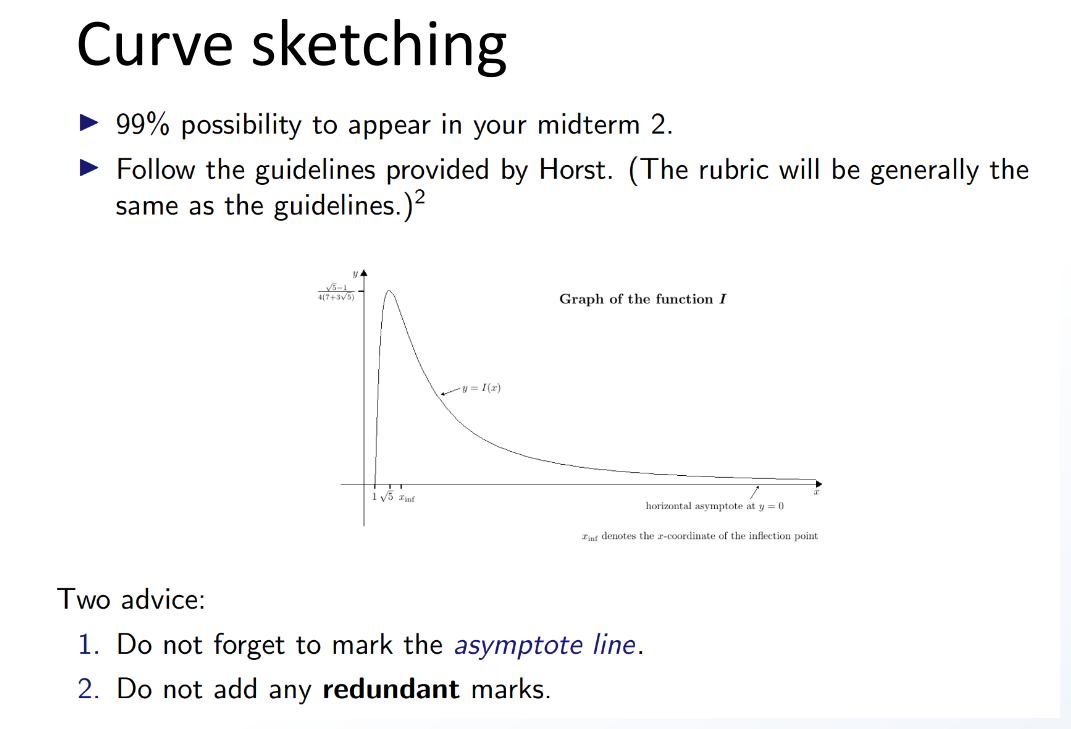
\includegraphics[width=11cm]{sketching.png}
    \end{figure}
\end{frame}

\section{Vector Space}
\begin{frame}
    \frametitle{Vector Space}

    \hspace{1em}By introducing vector space, one can treat a specific group of functions which all have some shared properties to form such a set, then
    we can find out some convenient operation that will make us easier to deal with them.\\
    \vspace{1em}
    \hspace{1em}
    We then make a specific definition to which \textbf{set} can be called a \textbf{Vector Space}.

\end{frame}

\begin{frame}
    \frametitle{Vector Space}

    We have eight axioms of vector space $V$ (in $\mathbb{C}$ or $\mathbb{R}$)\\

    \begin{center}
        $+:V\times V\rightarrow V$
    \end{center}

    \begin{enumerate}
        \item[i]    $(u+v)+w=u+(v+w)$
        \item[ii]   $u+v=v+u$
        \item[iii]  $\exists e\in V$ such that $v+e=e+v=v$
        \item[iv]   $\underset{v\in V}{\forall}\ \underset{(-v)\in V}{\exists}$ such that $v+(-v)=(-v)+v=e$
    \end{enumerate}

    \begin{center}
        $\cdot:\mathbb{F}\times V\rightarrow V$
    \end{center}

    \begin{enumerate}
        \item[i]    $1\cdot u=u\cdot 1=u$
        \item[ii]   $\lambda\cdot(u+v)=\lambda\cdot u+\lambda\cdot v$
        \item[iii]  $(\lambda+\mu)\cdot u=\lambda\cdot u+\mu\cdot u$
        \item[iv]   $(\lambda\mu)\cdot u=\lambda(\mu\cdot u)$
    \end{enumerate}

\end{frame}
\begin{frame}
    \frametitle{Vector Space}
    \begin{center}
        \center \textbf{Common Misunderstanding}
    \end{center}
    \vspace{1em}
    A real vector space is a subset of $\mathbb{R}^n$; a complex vector space is a subset of $\mathbb{C}^n$.\\
    \vspace{1em}
    \hspace{1em}
    When we say a vector space is real, or complex, we just refer to the \textcolor{blue}{scalar multiplication} – the scalar is real, or complex. We don’t set extra limitation on the element of the vector space.
    \begin{figure}
        \centering
        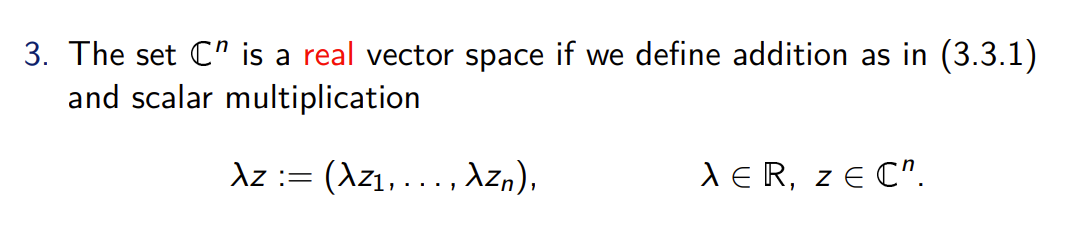
\includegraphics[width=1\textwidth]{real-vec.png}
    \end{figure}
\end{frame}

\begin{frame}
    \frametitle{Subspace}
    \hspace{1em}
    Let $(V,+,\cdot)$ be a real (complex) vector space and $U\subset V$. If $u_1+u_2\in U$ for $u_1,u_2\in U$, and $\lambda u\in U$ for all $u\in U$ and $\lambda \in \mathbb{F}$, then $(U,+,\cdot)$ is a
    subspace of $(V,+,\cdot)$.\\

    \hspace{1em}
    \begin{itemize}
        \item This lemma actually states that, when the maps “$+$” and “$\cdot$” makes sense in the subset $U$, then $U$ will \textcolor{blue}{inherit the eight axioms} of $V$.
        \item for a subspace, we don’t need to check the 8 axioms as they are
              inherited from the original vector space. Only check the addition and product is closed is enough.
    \end{itemize}


\end{frame}





\begin{frame}
    \frametitle{Recap: Metric}
    The definition of metric is as follows.
    \vspace{1em}
    \begin{itemize}
        \item $\forall x,y\in M,\ \rho (x,y) \geq 0$ and $\rho (x,y)=0$ if and only if $x=y$.
        \item  $\forall x,y\in M,\ \rho (x,y)=\rho (y,x)$.
        \item  $\forall x,y,z\in M,\ \rho (x,z)\leq \rho (x,y)+\rho (y,z)$
    \end{itemize}
    \hspace{1em}
    Since the metric measure the distance between two points(elements) in the set, now we want to directly measure the \textcolor{blue}{length} of one single element.\\
    \vspace{1em}
    \hspace{1em}
    We modified our length function as follows.
    \begin{itemize}
        \item Still positive, and equal to zero if and only if this \textcolor{blue}{vector} is 0 ($e$).
        \item \textcolor{blue}{Triangle inequality} still holds(with some modification).
        \item The \textcolor{blue}{symmetric} property makes no sense in this case, so\dots
    \end{itemize}

\end{frame}
\begin{frame}
    \frametitle{"Metric" in Vector Space}
    \begin{center}
        \hspace{1em} The \textcolor{blue}{symmetric} property makes no sense in this case, so\dots
    \end{center}

    \hspace{1em}Replace it by another important property in vector space. As you might notice, we care about \textcolor{blue}{scalar multiplication}, so the new property is
    \begin{center}
        The length of $\alpha u$?
    \end{center}

    \hspace{1em}Equal to $\alpha$ times the length of $u$
    ,where $u$ is a vector and $\alpha$ is a scalar. \\ \vspace{0.5em}\hspace{1em}Just as metric, we would like to give this function a name since it is so important,
    we will call it a \textbf{norm}. We then give the explicit definition of a norm.
\end{frame}

\section{Norm}
\begin{frame}
    \frametitle{Norm}
    \hspace{1em}
    Let $V$ be a real(complex) vector space. Then a map
    \begin{equation*}
        ||\cdot||:V\rightarrow \mathbb{R}
    \end{equation*}
    is called a norm if for all $u,v\in V$ and all $\lambda\in\mathbb{F}$, we have the following:
    \begin{itemize}
        \item $||\cdot||\geq 0$ for all $v\in V$ and $||v||=0$ if and only if $v=0$
        \item $||\lambda\cdot v||=|\lambda|\cdot ||v||$
        \item $||u+v||\leq ||u||+||v||$
    \end{itemize}
    \vspace{1em}
    Comment.  Obviously, any normed can be considered as a metric of that space. However, \emph{not} all the distance function generating metrics can be
    considered as a norm. A counterexample is:$\rho(x,y)=0$ if $x=y$ and $\rho(x,y)=1$ if $x\neq y$. The reason is when defining metric we don't assume
    the second property.

\end{frame}
\begin{frame}
    \frametitle{Norm}
    Examples\\

    \begin{itemize}
        \item $V=\mathbb{R}^n, ||(a_1,a_2,\dots,a_n)||=\sum^{n}_{k=1}|a_k|$
        \item $V=C[a,b], ||f||=\underset{x\in[a,b]}{\max}|f(x)|$
        \item $f:U\rightarrow V, ||f||=\underset{x\in U\backslash\{0\}}{\sup}\frac{||f(x)||_2}{||x||_1}$, where $||\cdot||_1$ is a norm defined on $U$ and $||\cdot||_2$ is a norm defined on $V$.
        \item $V=C[a,b], ||u||=\sup\{|u(z)|\cdot p(z):z\in[a,b]\}$, where $p$ is a real-valued function on $[a,b]$ and $0<\alpha\leq p(z)\leq \beta $ for some $\alpha,\beta>0$.
    \end{itemize}

    \vspace{1em}
    Comment. The third example is often called "\emph{operator norm}"; while the last example is often called "\emph{weighted norm}", a modification of which is useful in complex analysis.

\end{frame}
\begin{frame}
    \frametitle{More Examples in the Slides}
    \centering
    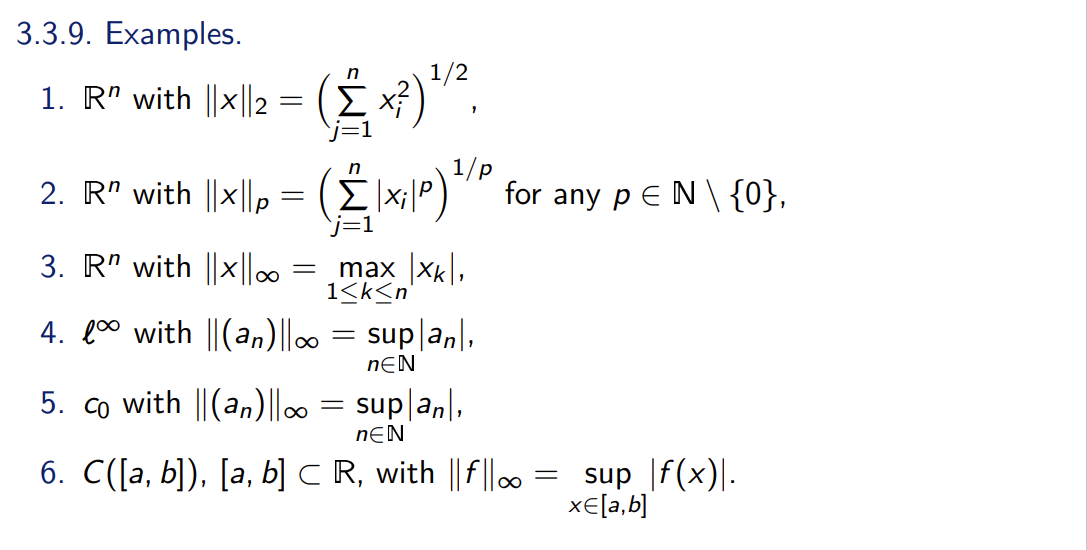
\includegraphics[width=1\textwidth]{example.png}

\end{frame}
\begin{frame}
    \frametitle{Exercise}
    1. Prove the (reverse) triangle inequality for a norm
    \begin{equation*}
        ||\cdot||:V\rightarrow \mathbb{R}.
    \end{equation*}
    That is, to prove
    \begin{equation*}
        |\ ||x||-||y||\ |\leq ||x\pm y||\text{, where }x,y\in V
    \end{equation*}
\end{frame}
\begin{frame}
    \frametitle{Exercise}
    2$^*$. Prove that a weighted norm is a norm
    on $C([a,b])$
\end{frame}
\begin{frame}
    \frametitle{Exercise}
    3. Check whether the following sentences are true or false:
    \begin{itemize}
        \item Given a vector space $V$, and its two non-empty subspaces $V_1, V_2$, then $V_1\cup V_2$ is a subspace of $V$.
        \item Given a vector space $V$, and its two subspaces $V_1,V_2$, then $V_1\cap V_2$ is a subspace of $V$.
        \item The set of all linear maps on $\mathbb{R}$ is a subspace of $C(\mathbb{R})$.
        \item Given a vector space $\mathbb{R}^n$, for any two distince norms $||\cdot||_1, ||\cdot||_2$ of $\mathbb{R}^n$, $||\cdot||:=\sqrt{||\cdot||_1\cdot||\cdot||_2}$ is also a norm of $\mathbb{R}^n$.
        \item Given a vector space $V$, given two norms $||\cdot||_1:V\rightarrow\mathbb{R}, ||\cdot||_2:\mathbb{R}\rightarrow\mathbb{R}$, then the $||\cdot||:=||\cdot||_2\circ||\cdot||_1$ is a norm of $V$.
    \end{itemize}
\end{frame}
\begin{frame}
    \frametitle{Convergence in Vector Space}
    Now we have our length function in the vector space, namely a norm. Then we can talk about the convergence and continuity in vector space. We start with convergence.\\
    \vspace{1em}
    \hspace{1em}
    Let $(V,||\cdot||)$ be a normed vector space. A sequence in $V$ is a map $(a_n):\mathbb{N}\rightarrow V$. We say that $(a_n)$ converges to $a\in V$ if
    \begin{equation*}
        \underset{\varepsilon>0}{\forall}\ \underset{N\in\mathbb{N}}{\exists}\ \underset{n>N}{\forall}\ ||a_n-a||<\varepsilon
    \end{equation*}

\end{frame}

\begin{frame}
    \frametitle{Continuity in Vector Space}
    Now let us introduce an interesting theorem. \\
    \vspace{1em}
    \hspace{1em}
    Let $(V,||\cdot||)$ be a normed vector space. The norm
    \begin{equation*}
        ||\cdot||:V\rightarrow \mathbb{R}
    \end{equation*}
    is a \emph{continuous} function on $V$.

    \vspace{1em}
    $Proof.$ \hspace{1em}
    By (reverse) triangle inequality,
    \begin{equation*}
        |\ ||x||-||y||\ |\leq ||x-y||.
    \end{equation*}

    Fix arbitrary $\varepsilon>0$, choose $\delta=\frac{1}{2}\varepsilon$ and we are done.
\end{frame}
\begin{frame}
    \frametitle{Exercise}
    5. Given a vector space $(V,||\cdot||)$.\\
    Let $a\in V$ be fixed; let $\lambda\neq 0\in \mathbb{F}$($\mathbb{C}$ or $\mathbb{R}$) be fixed. Prove the following.

    The scalar multiplication function $g:V\rightarrow V, g(x)=\lambda x$ is a continuous function and has a continuous inverse function.

\end{frame}

\begin{frame}
    \frametitle{Inner Product }
    Let $\mathbb{F}$ denote $\mathbb{R}$ or $\mathbb{C}$. An inner product in a real or complex vector space
    $V$ is a map $(x,y):V \times V \to \mathbb{F}$, such that the following holds:
    \begin{itemize}
        \item The inner product is linear in the first variable, i.e., for all $x, y, z \in V$ and all $\alpha, \beta \in \mathbb{F}, (\alpha x+\beta y,z)=\alpha(x,z)+\beta(y,z)$
        \item For all $x,y \in V$, $(x,y)=\overline{(y,x)}$ ̅if $V$ is complex,  and $(x,y)=(y,x)$ if $V$ is real.
        \item The inner product is positive definite, i.e., $(x,x)\geq 0$ for all $x$ and $(x,x)=0$ if and only if $x=0$
    \end{itemize}
    If a vector space $V$ is endowed with an inner product, we call it real
    (or complex) inner product space. If $V$ is a real inner product space,
    then $(x, \alpha y+\beta z)=(\alpha y+\beta z,x)=\alpha(y,x)+\beta (z,x)=\alpha (x,y)+\beta (x,z)$

\end{frame}

\begin{frame}
    \frametitle{Examples}
    \begin{itemize}
        \item $\mathbb{R}^n$ forms a real vector space with the inner product $$(\cdot~, ~\cdot):\R ^n \times \R^n \to \R ,~ (x,y)=\sum_{i=1}^n x_i y_i $$
        \item $\mathbb{R}^2$ forms a real vector space with the inner product $$(\cdot~, ~\cdot):\R^2 \times \R^2\to \R ,~ (x,y)=2x_1 y_1+x_1 y_2+x_2 y_1+2x_2 y_2$$
        \item $\mathbb{C}$ forms a complex vector space with the inner product $$(\cdot~, ~\cdot):\mathbb{C} \times \mathbb{C}\to \mathbb{C}, ~(x,y)=x \bar{y}$$
    \end{itemize}

\end{frame}

\begin{frame}
    \frametitle{Diagram}
    \begin{figure}
        \subfigure{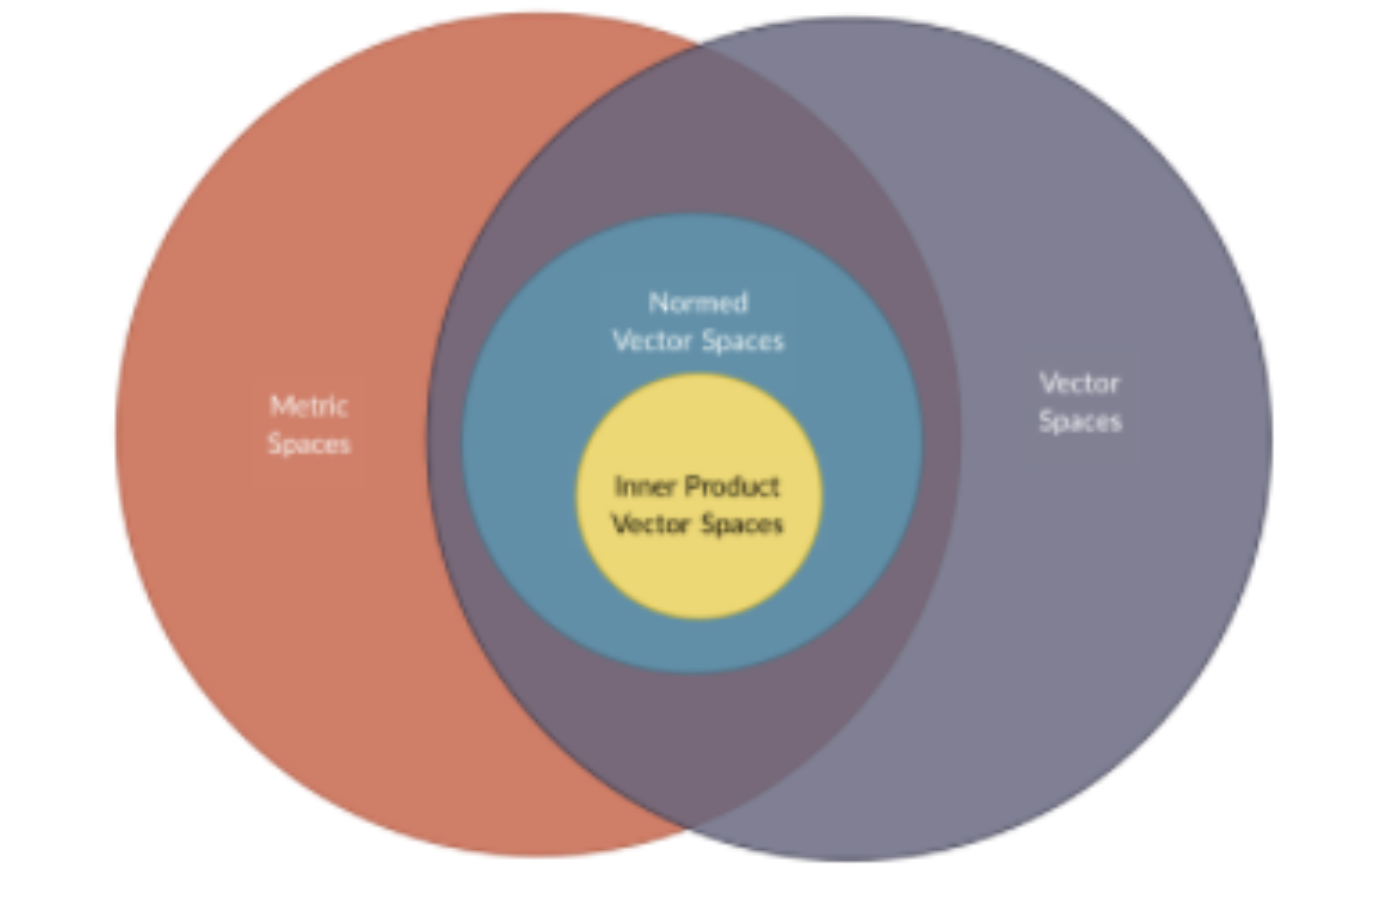
\includegraphics[width=0.9\textwidth]{space2.png}}
    \end{figure}


\end{frame}
\section{Function Sequences}
\begin{frame}
    \frametitle{Convergence of Function Sequences}
    Let $(f_n)$ be a sequence of real functions on $\Omega \subset \mathbb{R}$, then \\
    \begin{itemize}
        \item [1.]Pointwise convergence. For every $x \in \Omega,$ $$f_n (x) \xrightarrow{(n\to \infty)} f(x) ~~~~  :\Leftrightarrow ~~~~ |f_n ~(x)-f~(x)|\to 0$$
        \item [2.]Uniform convergence. $$f_n \xrightarrow{(n\to \infty)} f  ~~~~~:\Leftrightarrow ~~~~~  \underset{x \in \Omega}{\sup} ⁡|f_n (x)-f~(x)|\to 0 $$
    \end{itemize}

    Comment. For uniform convergence, we deal with the functions $f_n$ as a whole, instead of each $f_n (x)$;
    for pointwise convergence, we deal with function values. Uniform convergence automatically implies pointwise convergence
\end{frame}

\begin{frame}
    \frametitle{An example to illustrate Uniform Convergence \& Pointwise Convergence}
    \textcolor{red}{whether the N($\epsilon$) is related to x ? Or only related to $\epsilon$ ?}
    \begin{figure}[htbp]
        \centering
        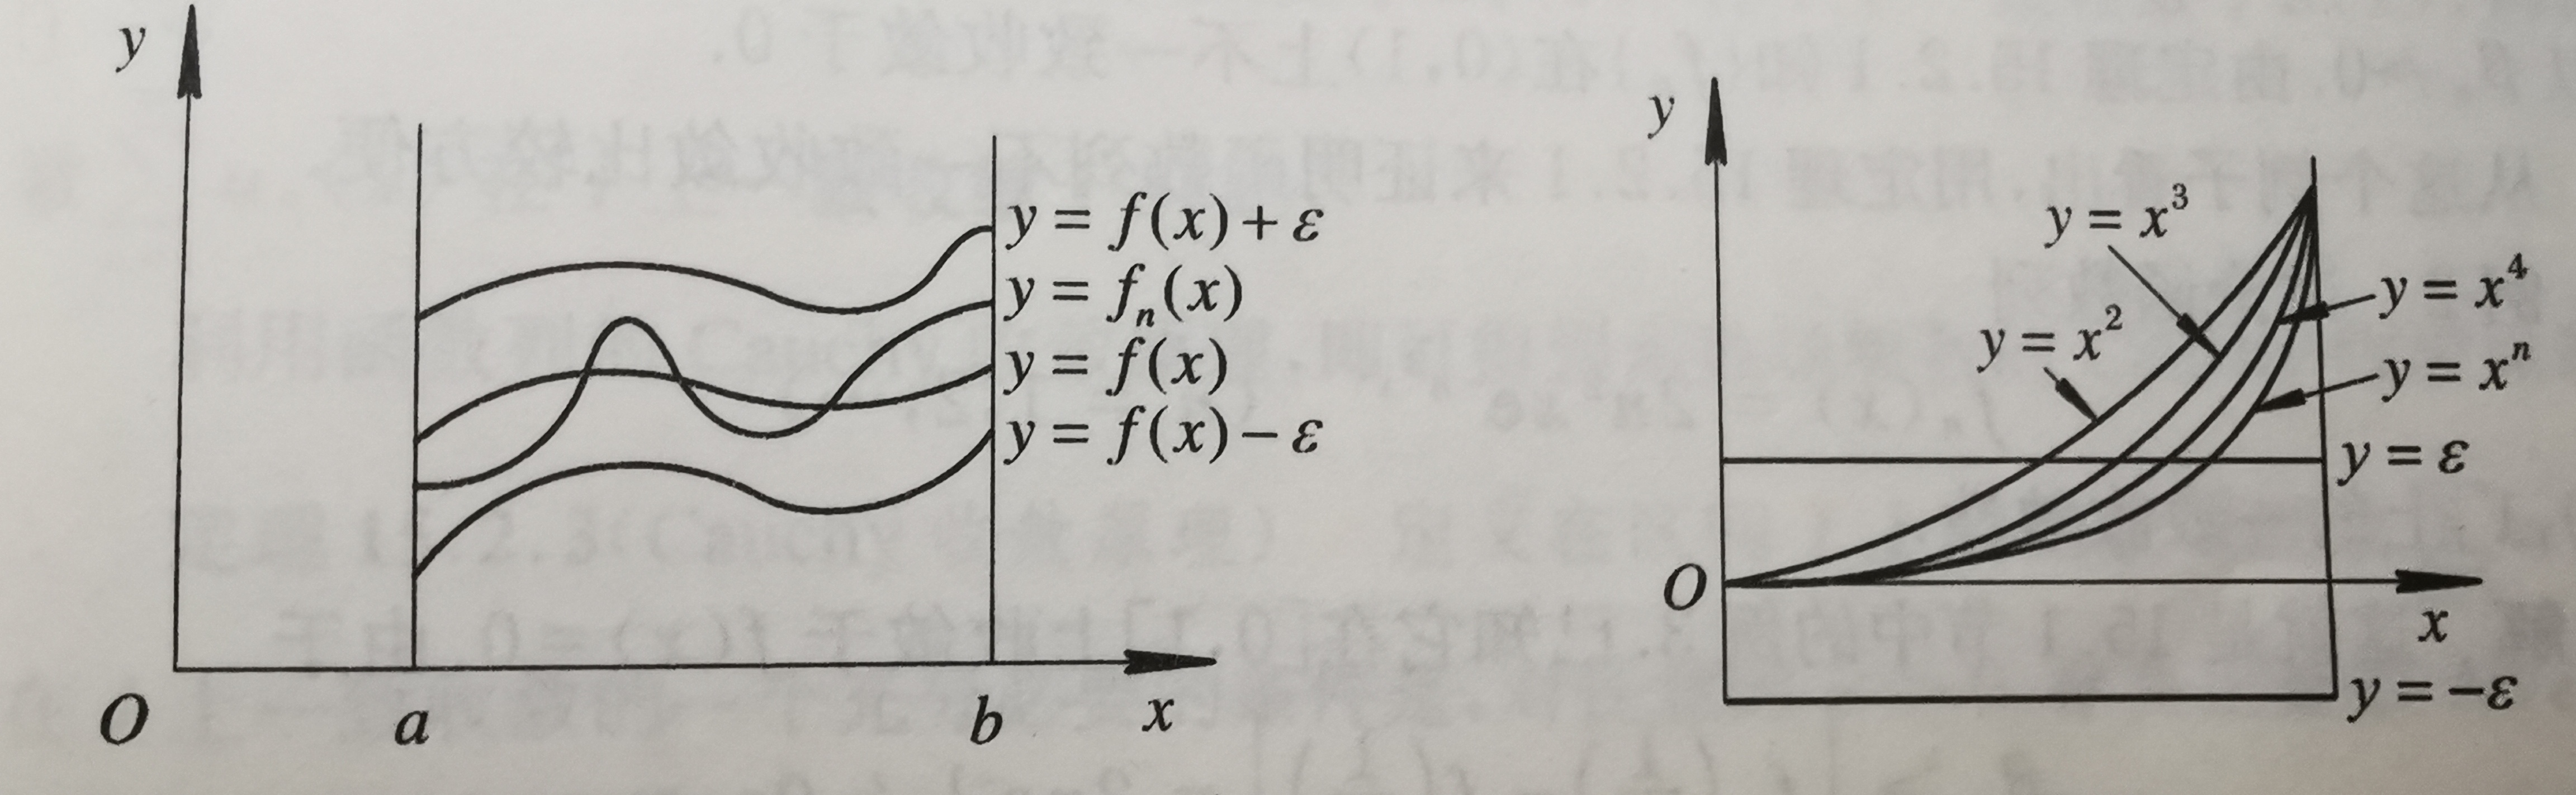
\includegraphics[width=12cm]{illustrate.jpg}
    \end{figure}
\end{frame}

\begin{frame}
    \frametitle{Example}
    \centering
    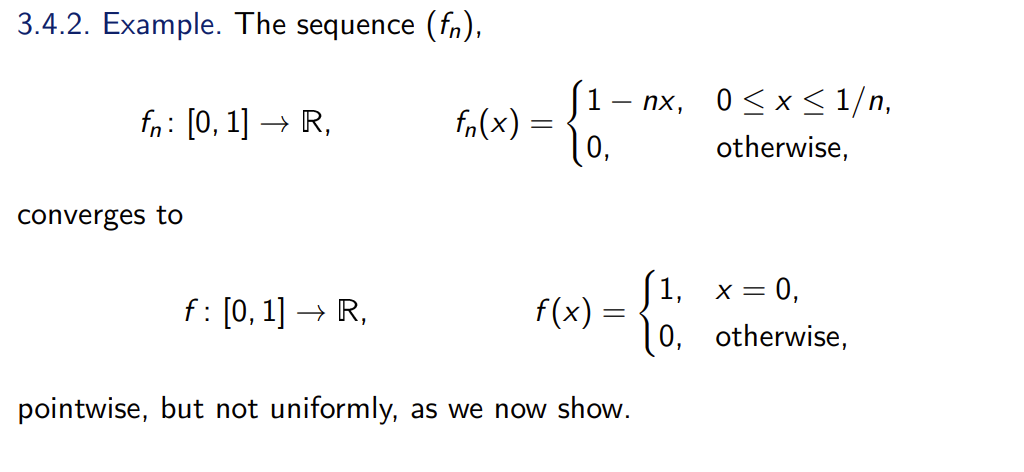
\includegraphics[width=1\textwidth]{seq_of_func.png}
\end{frame}
\begin{frame}
    \frametitle{How to find the limit}
    \hspace{1em}
    Since function vector space is abstract, we can use pointwise convergence
    to help us find the limit of a function sequence:\\
    \vspace{1em}
    \begin{itemize}
        \item [1.]Calculate the pointwise limit $f$ of a given function sequence $(f_n)$.
        \item [2.] Find a formula or estimate of $||f_n - f||$ for any $ n \in \mathbb{N} $.
        \item [3.] If $||f_n - f|| \to 0$ as $n \to \infty$, then $(f_n)$ converges uniformly to $f$.
              Otherwise the convergence is not uniform.
    \end{itemize}

\end{frame}
\begin{frame}
    \frametitle{Exercise}
    7. Calculate the limit of $(f_n)$, sketch their graph, and
    determine whether the convergence is uniform or not.
    \begin{itemize}
        \item   $f_n:\mathbb{R}\to \mathbb{R}, f_n (x)=\frac{(|x|^n)}{(1+|x|^n )}, n \in \mathbb{N}$\\
              \vspace{1em}
        \item  $f_n:\mathbb{R}\to \mathbb{R},f_n (x)=\sqrt{x^2+\frac{1}{n^2}}, n \in \mathbb{N} $
              \vspace{1em}
        \item $f_n: \mathbb{R} \to \mathbb{R}, f_n (x)=\frac{x^2+n x}{n}, n \in \mathbb{N}^*$
    \end{itemize}
\end{frame}

\begin{frame}
    \frametitle{Exercises}
    8. Let $(f_n)$ be a sequence of functions in $C([a,b])$,
    and $(f_n)$ converges to some function $f$ uniformly.
    Prove that if $f\neq 0$ on $[a,b]$, then $(\frac{1}{f_n} )$ converges to $\frac{1}{f}$ uniformly.
\end{frame}

\begin{frame}
    \textcolor{red}{Important Theorem \& Learn The Proof}
    \begin{figure}[htbp]
        \centering
        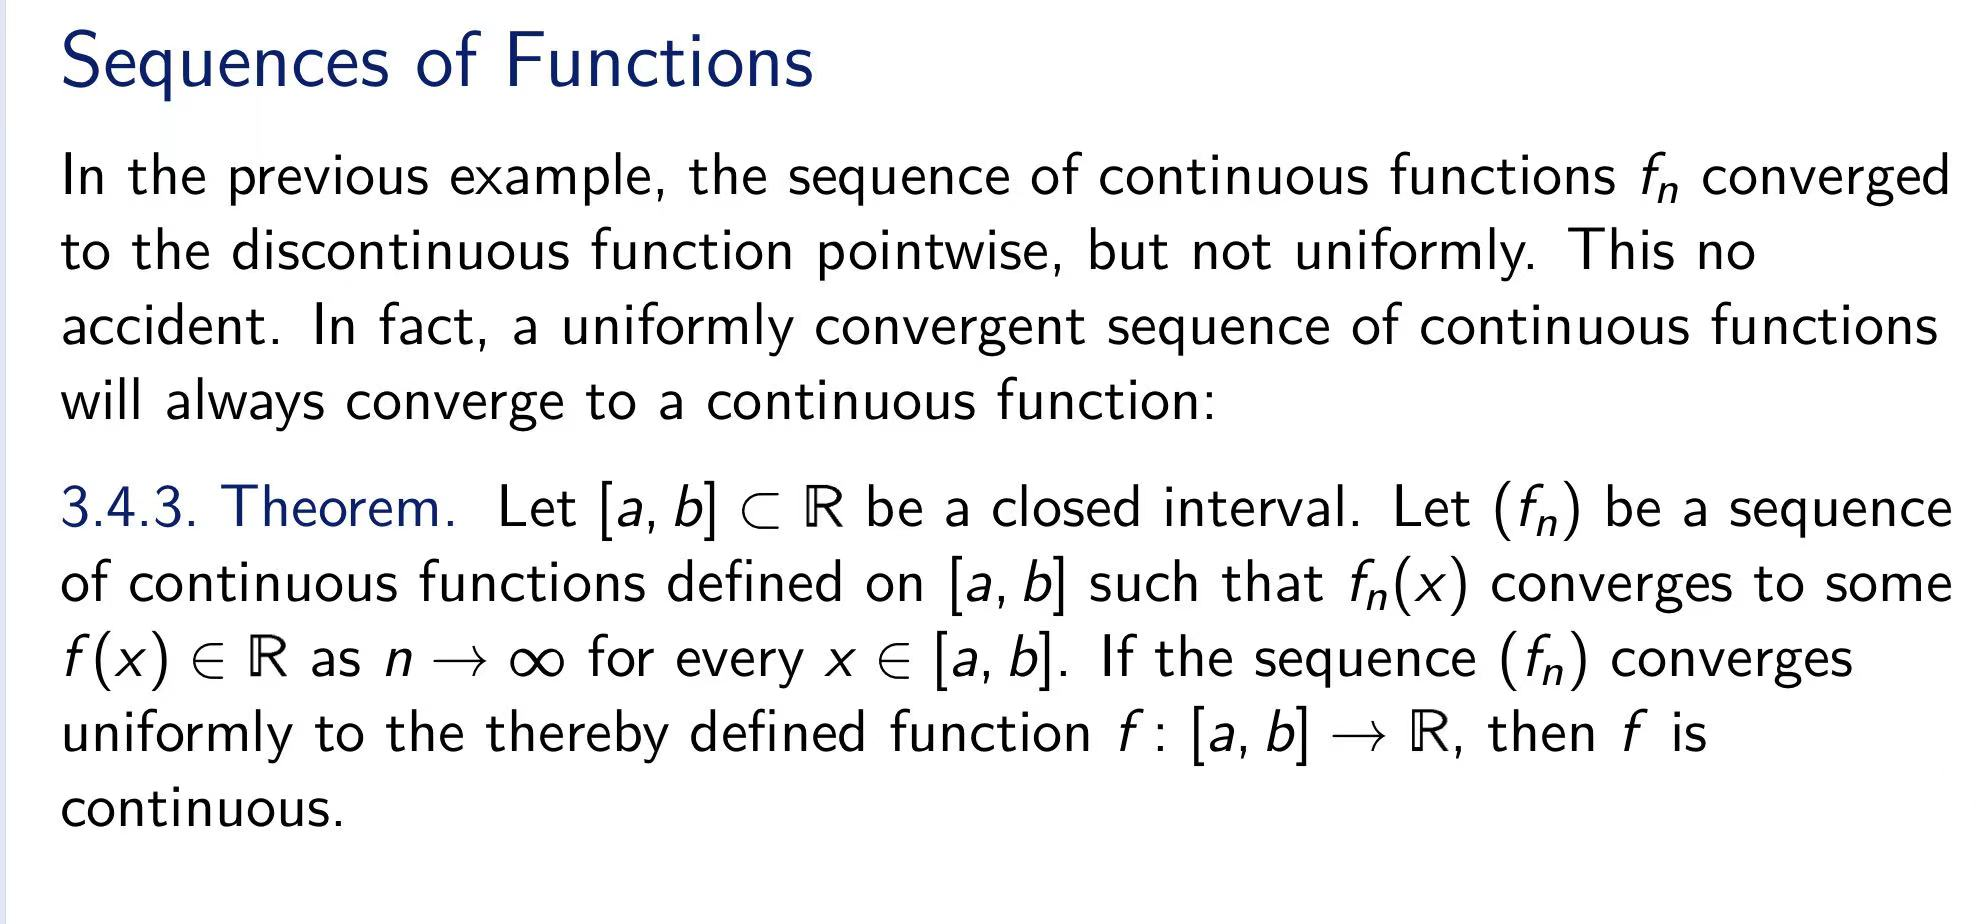
\includegraphics[width=10cm]{important1.jpg}
    \end{figure}
\end{frame}

\begin{frame}
    \begin{figure}[htbp]
        \centering
        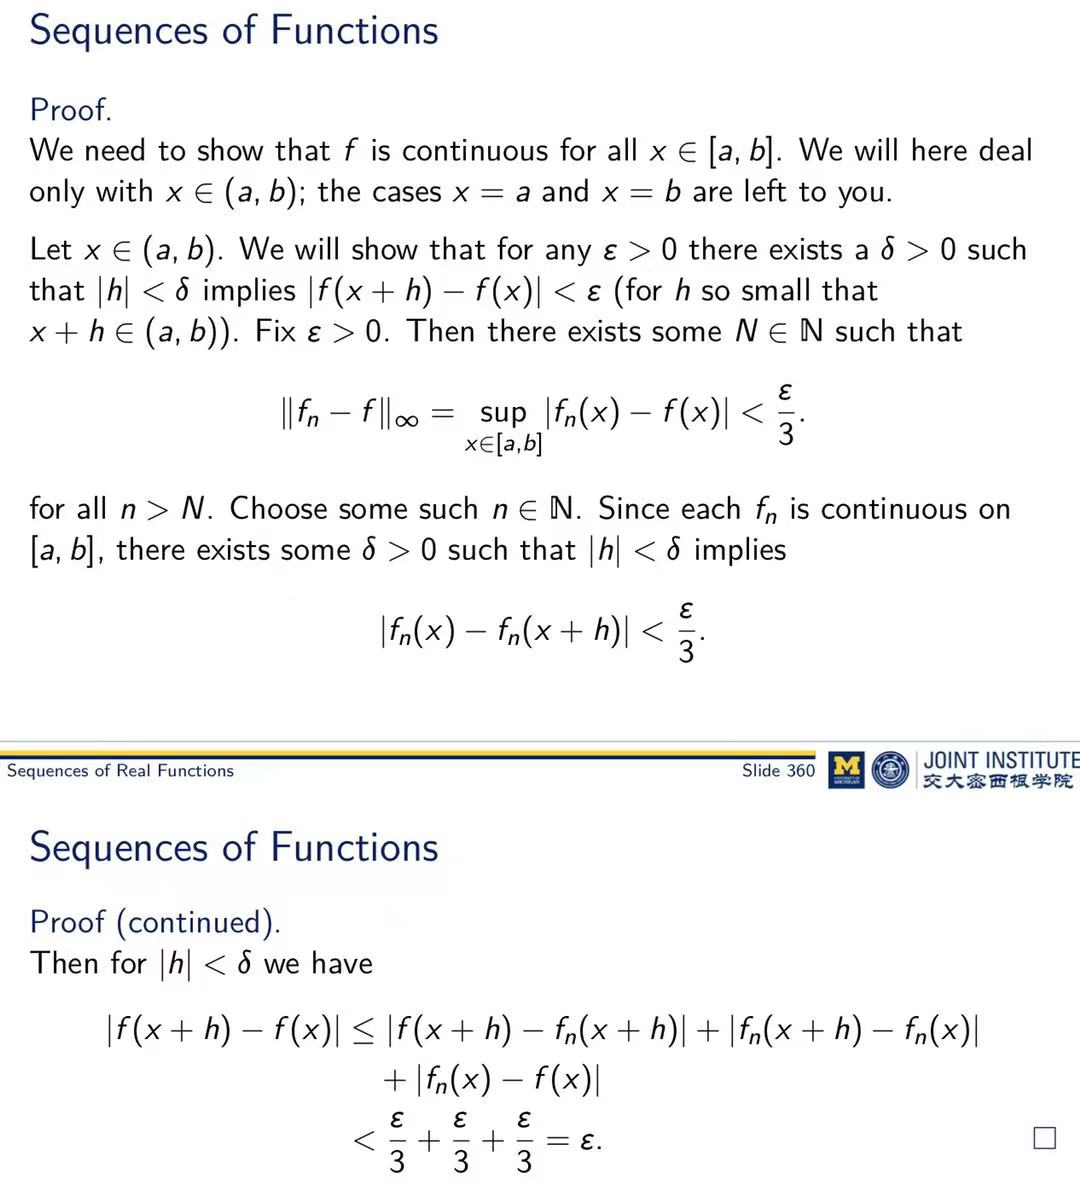
\includegraphics[width=7cm]{important2.jpg}
    \end{figure}
\end{frame}

\begin{frame}
    \frametitle{\textcolor{red}{Challenging}}
    9$^*$.$(f_{n})$ is a sequence of increasing functions, $f_{n}$:[0,1]$\rightarrow$[0,1] is pointwise convergent.
    Suppose f is continuous, show uniform convergence.
\end{frame}

\begin{frame}
    \frametitle{Exercises}
    10$^*$.Let $(f_n )$ be a sequence of functions such that for each $n\in \mathbb{N}$,
    $f_n  \in C([a,b])$, $\forall x \in [a,b]$,  $(f_n (x))$ is a bounded monotonic sequence.\\
    \vspace{1em}
    \begin{itemize}
        \item Please show that $(f_n)$ converges point-wisely to some function $f$
        \item Suppose $f \in C([a,b])$, prove that $(f_n )$ converges uniformly to $f $
    \end{itemize}

\end{frame}


\begin{frame}
    \frametitle{Reference}
    \begin{itemize}
        \item Many Contents from 2021-Vv186TA Niyinchen
    \end{itemize}
\end{frame}
\begin{frame}
    \frametitle{End}
    \centering
    \LARGE{Thanks!}


\end{frame}
\end{document}